\hypertarget{introduction-into-software-evolution}{%
\section{Introduction into Software
Evolution}\label{introduction-into-software-evolution}}

\begin{tcolorbox}[colback=blue!5!white,colframe=blue!75!black]
You
\begin{itemize}
\tightlist
\item
  understand and can explain the need for software change
\item
  understand how an evolutionary software process supports constant
  change
\item
  can explain the challenges of legacy systems
\item
  know methods, tools and practices for an evolutionary software
  development
\item
  know current trends in software evolution
\end{itemize}
\end{tcolorbox}

\hypertarget{software-maintenance}{%
\subsection{Software Maintenance}\label{software-maintenance}}

Classification of software maintenance activities:

\begin{itemize}
\tightlist
\item
  Corrective: errors need to be fixed.
\item
  Preventive: prevent problems in the future (fix design issues).
\item
  Adaptive: something has changed in the environment.
\item
  Perfective: improve system qualities, e.g.~performance.
\end{itemize}

\hypertarget{but-why}{%
\subsubsection{But why?}\label{but-why}}

\begin{tcolorbox}[colback=red!5!white,colframe=red!75!black]
Programs, like people, get old. We can’t prevent aging, but we can understand its causes
\end{tcolorbox}

\begin{figure}[H]
\centering
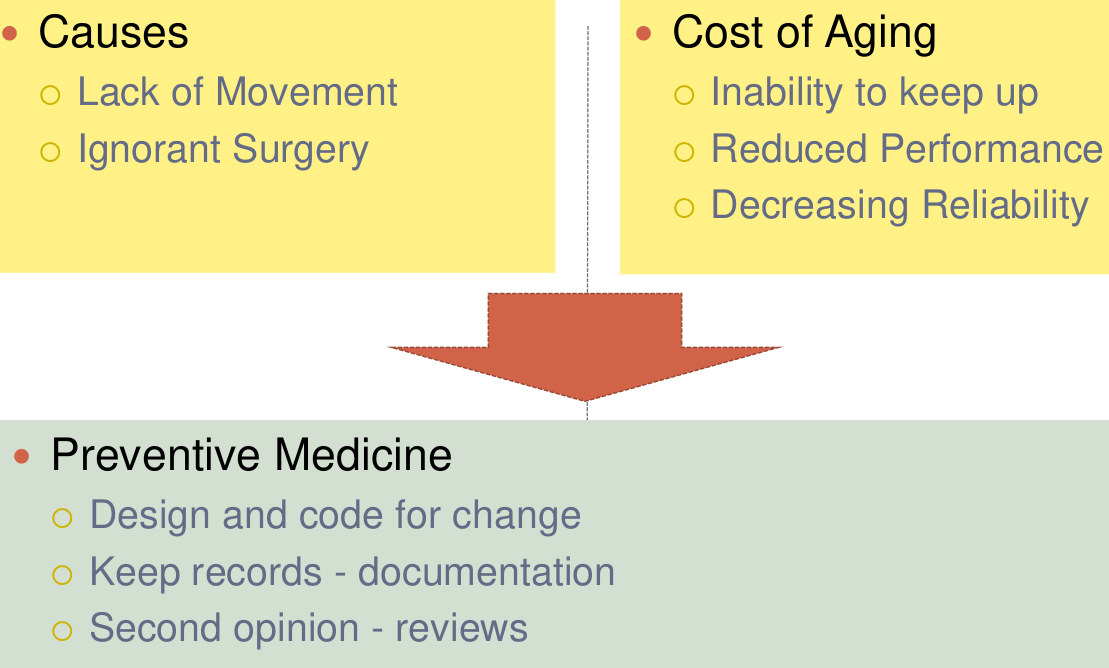
\includegraphics[width=0.5\textwidth]{figures/softwareAging.png}
\caption{Code Aging}
\end{figure}

\hypertarget{Causes of Software Aging}{%
\subsubsection{Causes of Software Aging}\label{Causes-of-Software-Aging}}
\begin{itemize}
    \item Lack of Movement
    \subitem Caused by Product owner for not seeing the need for change
    \subitem   Unless software is frequently updated, its users will become
  dissatisfied and they will change to a new product as soon as the
  benefits outweigh the costs of retraining and converting.
  
  \item Ignorant Surgery
  \subitem Small changes made to software by people who do not understand the design. This degrades the structure of the program. Without Testing.
  \subitem Software that has beed repeadedly modified in this way becomes very expensive to update.
\end{itemize}

\hypertarget{Symptoms of Software Aging}{%
\subsubsection{Symptoms of Software Aging}\label{Symptoms-of-Software-Aging}}
\begin{itemize}
    \item Owners find it hard to keep up with the marked
    \item Software degrades due to weak strukture
    \item Software becomes buggy.
\end{itemize}


\hypertarget{maintenance-vs.evolution}{%
\subsubsection{Maintenance
vs.~Evolution}\label{maintenance-vs.evolution}}

\begin{itemize}
\tightlist
\item
  Software maintenance = the activities of changing the system after it
  has been delivered
\item
  Software evolution = the process of continuous software change from
  the very beginning

  \begin{itemize}
  \tightlist
  \item
    Development activities + Maintenance activities + Reengineering
    activities
  \end{itemize}
\end{itemize}

\hypertarget{importance-of-evolution}{%
\subsection{Importance of Evolution}\label{importance-of-evolution}}

\begin{itemize}
\tightlist
\item
  Organizations have huge investments in their software systems - they
  are critical business assets.
\item
  To maintain the value of these assets to the business, they must be
  changed and updated.
\item
  The majority of the software budget in large companies is devoted to
  evolving existing software rather than developing new software.
\item
  Studies indicate that up to 75\% of all software professionals are
  involved in some form of maintenance/evolution activity
\end{itemize}

\begin{figure}[H]
\centering
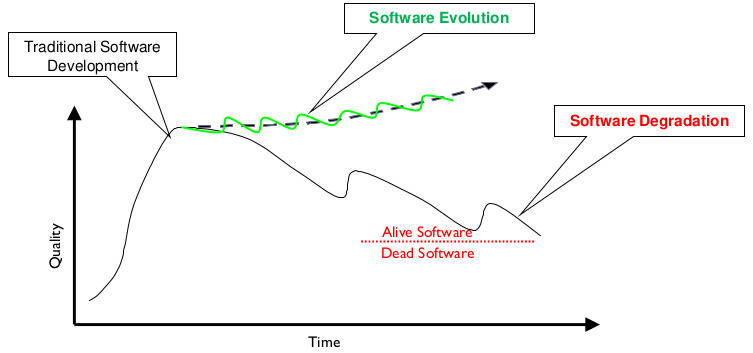
\includegraphics[width=0.5\textwidth]{figures/softwareEvolution.png}
\caption{Software evolution}
\end{figure}


\hypertarget{lehmans-laws-of-evolution}{%
\subsubsection{Lehman`s „Laws`` of
Evolution}\label{lehmans-laws-of-evolution}}
After serveral studies had similarities, Lehman decided to start write down the laws of software evolution to achieve a generatalisation in software behavior. The rules have to be applied that the software will survive. See Homework 1.

\begin{itemize}
\tightlist
\item
  Propose a theoretical model to reason about software systems and their
  interaction with the socio-economic environment.
\item
  Propose a classification of software: S-Programs, P-Programs and
  E-Programs.
  
\item 
Software has to evolve, otherwise the quality decreases and it becomes useless.


\begin{figure}[H]
\centering
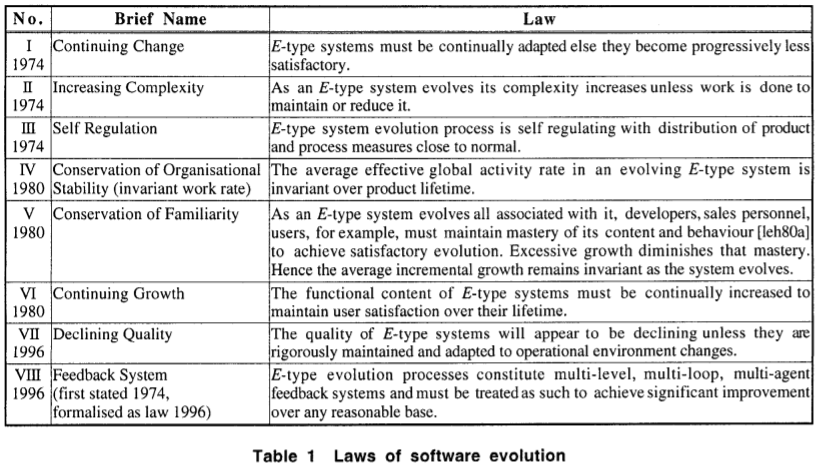
\includegraphics[width=0.5\textwidth]{figures/LehmansLaw.png}
\caption{Lehmans Laws}
\end{figure}


  \begin{itemize}
  \tightlist
  \item
    S-Programs. Programs that can be completely and formally specified.

    \begin{itemize}
    \tightlist
    \item
      e.g.~a program that sorts an array.
    \end{itemize}
  \item
    P-Programs. Programs that can be completely specified, but which
    makes an approximation of the real world.

    \begin{itemize}
    \tightlist
    \item
      e.g.~a program that plays chess against a human player.
    \end{itemize}
  \item
    E-Programs. Programs that mechanize a human or societal activity.
    The program becomes a part of the world it models!

    \begin{itemize}
    \tightlist
    \item
      e.g.~an ERP system.
    \end{itemize}
  \end{itemize}
\end{itemize}

\begin{tcolorbox}[colback=red!5!white,colframe=red!75!black]
Software systems have to evolve, otherwise they gradually become useless.

If you don’t take specific actions, software will become more complex and more difficult to adapt.
\end{tcolorbox}


\subsection{Evolution vs. Classical Approach}
In Classical Software Approach one used the waterfall model. It is a linear approach to develop Software. It is built up on different Project phases with milestones at the end. It is not Iterative. Whereas Software Evolution is a set of activities (technical and managerial), that ensures that software continues to meet organizational and business objects in a cost effective way over its lifetime. Changes are driven by the stakeholders.
\begin{figure}[H]
\centering
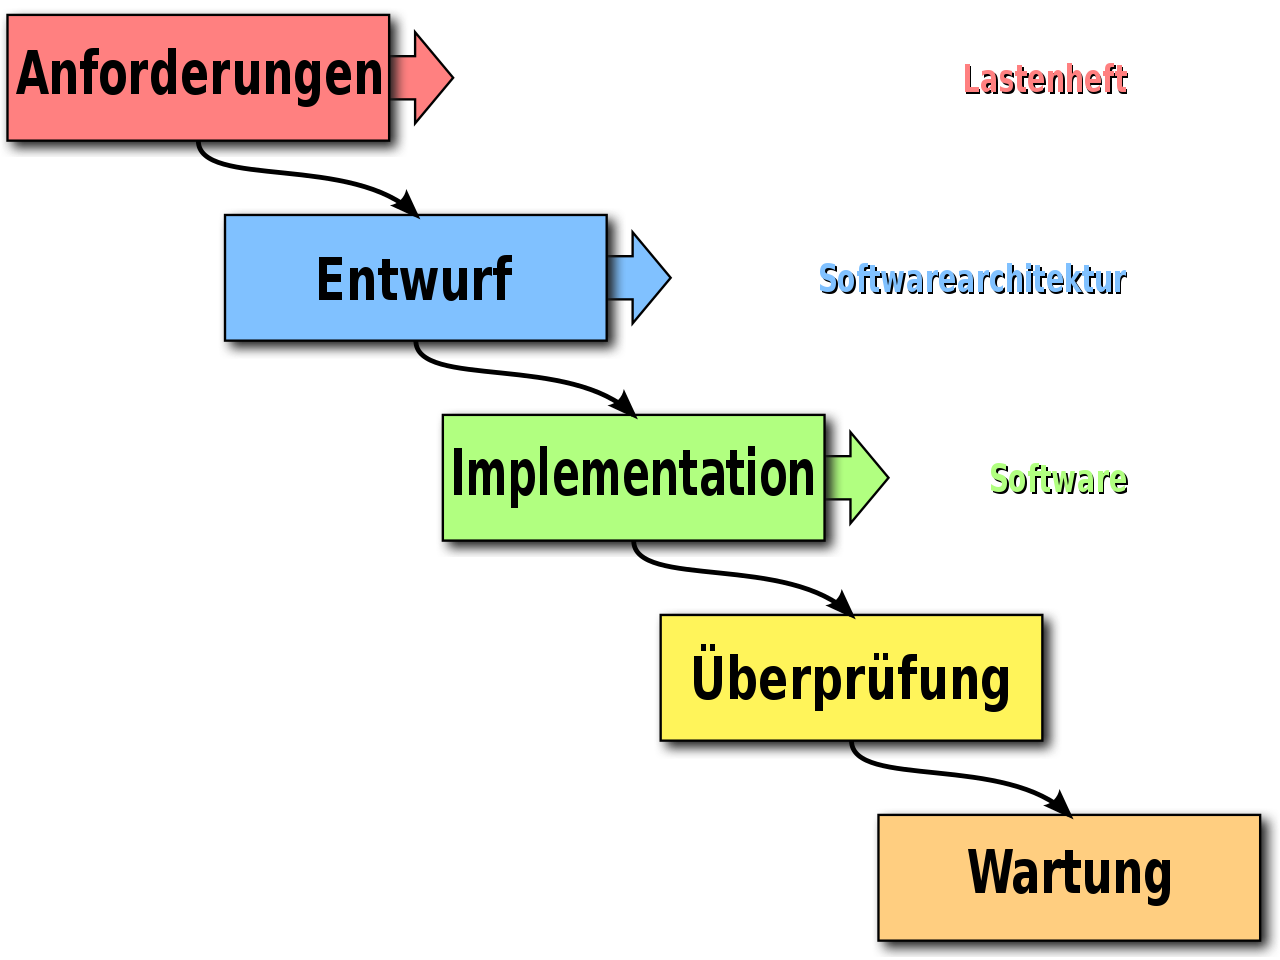
\includegraphics[width=0.5\textwidth]{figures/Waterfall.png}
\caption{Waterfall Model}
\end{figure}

\hypertarget{legacy-systems}{%
\subsection{Legacy Systems}\label{legacy-systems}}






\begin{tcolorbox}[colback=red!5!white,colframe=red!75!black]
Legacy systems: old computer-based systems, which are still in use by organizations
--> Have to be maintained!
\end{tcolorbox}

\begin{itemize}
\tightlist
\item
  For many systems, the software evolution process is not as
  straightforward as described.
\item
  Legacy systems are old systems that have become significantly
  difficult to modify.
\item
  Two complementary techniques are employed to support the continued
  evolution of legacy systems: Reverse engineering and Reengineering
\end{itemize}

\clearpage